\section{牛顿力学的一些简单应用}\label{sec:03.05}

\example 已知一个10千克的力$ F $水平地作用于质量为$ M = 6 0 $
千克的物体上,并通过它推另一质量为$ k = 4 0 $千克的物体
(图\ref{fig:03.08})。$ m $与$ M $都在水平面上,求:

(1) 设平面与物体之间无摩擦力,$ M $作用于$ m $上的力多大?

(2) 若$ m $的左边紧靠着一堵墙,$ M $作用在$ m $上的力有多大?

(3) 设$ M $与$ m $同水平面之间的摩擦系数分别为$ \mu _ { 1 } = 0 . 0 5 $ 和
$ \mu _ { 2 } = 0 . 1 0 $,$ M $作用于$ m $上的力又有多大?
\begin{figure}[!h]
    \centering
 \subfigure[]{
 \label{fig:03.08a}
 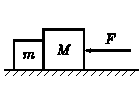
\includegraphics{figure/fig03.08a}
 }
 \subfigure[]{
 \label{fig:03.08b}
 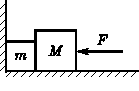
\includegraphics{figure/fig03.08b}
 }
 \subfigure[]{
 \label{fig:03.08c}
 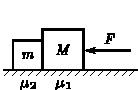
\includegraphics{figure/fig03.08c}
 }
 \caption{}
 \label{fig:03.08}
\end{figure}

% 101.jpg
\solution (1) 设$ M $与$ m $的加速度为$ a $它们之间的相互作用力为
$f_1$,则$ M $及$ m $的受力情况如图\ref{fig:03.09} 所示,它们的牛顿方程分别
为:
\begin{wrapfigure}[8]{r}{12em}
    \centering
    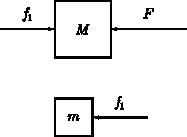
\includegraphics{figure/fig03.09}
    \caption{}
    \label{fig:03.09}
\end{wrapfigure}
\vspace{-1.4em}
\begin{align*}
 &F - f _ { 1 } = M a _ { 1 } \\
 &f _ { 1 } = m a _ { 1 }
\end{align*}
解之得
\begin{align*}
 f _ { 1 } &= \frac { M F } { m + M } \\
  &=4\text{千克力} < F
\end{align*}

(2) 因为$ m $紧靠墙,故$ a _ { 2 } = 0 $,所以
\begin{equation*}
 F - f _ { 2 } = 0
\end{equation*}
因此得
\begin{equation*}
 f _ { 2 } = F = 1 0 \text{千克力}
\end{equation*}

\begin{wrapfigure}[5]{r}{14em}
    \centering
    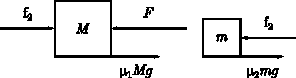
\includegraphics{figure/fig03.10}
    \caption{}
    \label{fig:03.10}
\end{wrapfigure}
(3) 受力情况如图\ref{fig:03.10}~所示,M及m的牛顿方程分别为:
{\setlength{\mathindent}{2em}
\begin{align*}
 &F - f _ { 3 } - \mu _ { 1 } M g = M a _ { 4 } \\
 &f _ { 3 } - \mu _ { 2 } m g = m a _ { 2 }
\end{align*}}
解之得
\begin{align*}
 f _ { B } &= \frac { m \left( F - \mu _ { 1 } M g \right) + \mu _ { 2 } m M g } { M + m } \\
  &= \frac { m F + m M g \left( \mu _ { 2 } - \mu _ { 1 } \right) } { M + m } \\
  &= 5.2 \text{千克力} < F
\end{align*}

\example 已知两个质量同为1公斤的物体用轻的弹簧连接在一
起,竖直地放在水平桌面上,如图\ref{fig:03.11}~所示。求:

(1)开始时两物都静止,将桌面突然移掉,在这一瞬间两物体
的加速度各为多少?
% 102.jpg

\begin{wrapfigure}[10]{r}{16em}
    \centering
    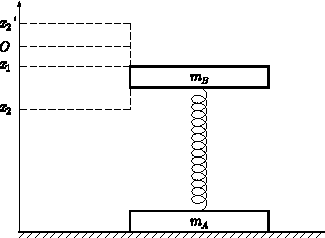
\includegraphics{figure/fig03.11}
    \caption{}
    \label{fig:03.11}
\end{wrapfigure}
(2)在$ m $上加多大压力,并保持其静止,才能使当压力突然撤去时,由
于弹簧的反跳导致$ m_B $刚刚离开面桌?

\solution (1)平衡时对于$ m_A $,重力$ W _ { A } = m _ { A } g $,是
向下的;弹簧的伸张力$ N _ { A } $是向上的,故静力平衡方程为:\vspace{-0.5em}
\begin{equation*}
	W _ { A } - N _ { A } = 0
\end{equation*}
或\vspace{-1.56em}
\begin{equation*}
	W _ { A } = N _ { A } = m _ { A } g
\end{equation*}
对于$ m_B $,重力$ W _ { B } = m _ { B } g $,是向下的3弹簧的伸张力为$ N _ { B } $; ,
也是向下的;桌面的支持力$ R $是向上的。故静力平衡方程为:
\begin{equation*}
	W _ { B } + N _ { B } = R
\end{equation*}
由于弹簧向上下的伸张力相同,则有
\begin{equation*}
	N _ { A } = N _ { B }
\end{equation*}
突然撤去桌面,故$  R = 0  $,这时,物体$ A $受到的总力为$  F _ { A } =
\sum _ i F _ { A _ i } = W _ { A } - N _ { 4 } = 0  $,即加速度为
\begin{equation*}
	a = 0
\end{equation*}
物体B受的总力为
\begin{align*}
	F _ { B } &= \sum _ i F _ { B _ i } \\
		&= W _ { B } + N _ { B } = m _ { B } g + m _ { A } g
\end{align*}
故加速度为
\begin{equation*}
	a _ { R } = \frac { m _ { A } + m _ { B } } { m _ { B } } g = 2 g
\end{equation*}

(2)如图\ref{fig:03.11}~所示,弹簧原长在$ O $点,加$ m_{A} $后压缩至$ x_{1} $
% 103.jpg

\noindent 点,再加压力$ P $后压缩至$ x_{2} $点。因为弹簧反跳的距离等于被压缩的
距离,所以撤去压力$ P $后弹簧到达的最高点为$  x'_ { 2 }  $,并且
\begin{equation*}
	\overline{ x _ { 1 } x _ { 2 } \llap{\phantom{'}} } = \overline{ x _ { 1 } x' _ { 2 }}
\end{equation*}
若要求$ m_B $能离开桌面,应有
\begin{equation*}
	k \overline{ O x' _ { 2 } } \geqslant m _ { B } g
\end{equation*}
其中为弹簧的倔强系数。因而,压力至少应为
\begin{align*}
	P &= k \overline{ x _ { 1 } x _ { 2 } \llap{\phantom{'}}} \\[-0.5em]
	  &= k \overline{ x _ { 1 } x ' _ { 2 } } \\[-0.5em]
	  &= k \left( \overline{ x _ { 1 } O \llap{\phantom{'}} } + \overline{ O x ' _ { 2 } } \right) \\[-0.5em]
	  &= k \overline { x _ { 1 } O \llap{\phantom{'}}} + k \overline { O x '_2} \\[-0.5em]
	  &\geqslant m _ { A } g + m _ { B } g
\end{align*}
所以,当$  P \geqslant \left( m _ { A } + m _ { B } \right) g = 2 \text{公斤力} $时,可使$ m_{B} $离开桌面。

\begin{wrapfigure}[8]{r}{15em}
    \centering
    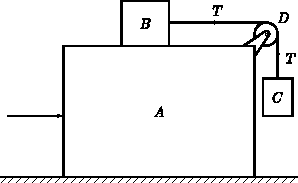
\includegraphics{figure/fig03.12}
    \caption{}
    \label{fig:03.12}
\end{wrapfigure}
\example 如图\ref{fig:03.12}~的装置,设各接触面都是光滑
的,定滑轮$ D $及绳的质量可忽略不计,绳不可伸长。要
使$ B $,$ C $相对$ A $为静止,应用多大的力$ F $推动整个装置?

\solution 整个装置及$ C $,$ B $的牛顿方程分别为
\begin{align*}
	&F = \left( m _{A} + m _ { B } + m _ { C } \right) a \\[-0.5em]
	&T - m _ { C } g = 0 \\[-0.5em]
	&T = m _ { B } a
\end{align*}
求解得到\vspace{-1.56em}
\begin{equation*}
	F = \left( m _ { A } + m _ { B } + m _ { C } \right) \frac { m _ { C } } { m _ { B } } g
\end{equation*}
其中$ m_{A} $,$ m_{B} $,$ m_{C} $相应为$ A $,$ B $,$ C $的质量。


\example 对于图\ref{fig:03.13a}~表示的体系,劈形物固定,两侧面光

% 104.jpg
\noindent 滑。若$  m _ { 1 } = 8 0 \text{克} $,$ m _ { 2 } = 1 0 0 \text{克} $,绳及定滑轮质量都可以忽略,绳也不可伸长。求

(1) 绳中张力$ T $及两物体的加速度。

(2) 两物体自静止开始运动后第二秒末绳忽然断掉,求绳断
后再过多久,又开始下滑?
\begin{figurex}
    \centering
    \subfigure[]{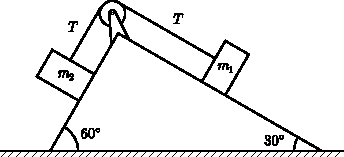
\includegraphics{figure/fig03.13a} \label{fig:03.13a}}\\[-0.5em]
    \subfigure[]{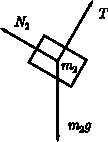
\includegraphics{figure/fig03.13b} \label{fig:03.13b}} \qquad
    \subfigure[]{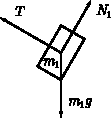
\includegraphics{figure/fig03.13c} \label{fig:03.13c}}
    \caption{}
    \label{fig:03.13}
\end{figurex}

\solution $m_1$,$m_2$各受三个力,即重力,斜面支持力及绳子的张力
\lhbrak 图\ref{fig:03.13b}及\subref{fig:03.13c}\rhbrak。

(1) $m_1$及$m_2$在运动方向上相应的牛顿第二定律表达式为
\begin{align*}
	T - m _ { 1 } g \sin 3 0 ^ { \circ } &= m _ { 1 } a \\[-0.5em]
	m _ { 2 } g \sin 6 0 ^ { \circ } - T &= m _ { 2 } a
\end{align*}
求解得到
\begin{align*}
	a &= \frac { m _ { 2 } \sin 6 0 ^ { \circ } - m _ { 1 } \sin 3 0 ^ { \circ } } { m _ { 1 } + m _ { 2 } } g = 2 . 5 3 \text{米/秒}^2 \\[-0.5em]
	T &= m _ { 1 } g \sin 3 0 ^ { \circ } - m _ { 1 } a = 5 . 9 5 \times 1 0 ^ { 4 } \text{达因}
\end{align*}

(2) 第二秒末的速度为

% 105.jpg
~\vspace{-1.56em}
\begin{equation*}
	v = a \times 2 = 2 . 5 3 \times 2 = 5 . 0 6 \text{米/秒}
\end{equation*}
绳断后,依靠惯性还要继续以匀减速度向上运动,直减至速度为
零才开始下滑。因减速度大小为$  g \sin 3 0 ^ { \circ } $故向上运动的时间为
\begin{equation*}
	t = \frac { v } { g \sin 3 0 ^ { \circ } } = 1 . 0 3\text{秒}
\end{equation*}

\example 一固定于桌面上的斜面(图\ref{fig:03.14a}),其中$  A B = 1 3 0  $
厘米,$  A C = 5 0  $厘米,滑块$  m _ { 1 } = 2 0 0  $克,$  m _ { 2 } = 6 0  $克,静置在斜面上。
两滑块间的静摩擦系数$  \mu _ { 0 } = 0 . 5 0 $ ,$m_2$与斜面间的滑动摩擦系数
$ \mu = 0 . 3 3  $,用平行于斜面的力$ F $向上拉$m_2$。求:

(1) 当$m_1$开始在$m_2$上滑动时,$m_2$的加速度等于多少?

(2) 上述滑动开始时的$ F $等于多少?
\begin{figurex}
	\centering
	\subfigure[]{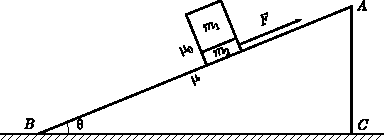
\includegraphics{figure/fig03.14a} \label{fig:03.14a}}\\[-0.5em]
	\subfigure[]{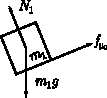
\includegraphics{figure/fig03.14b} \label{fig:03.14b}} \qquad
	\subfigure[]{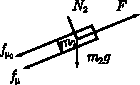
\includegraphics{figure/fig03.14c} \label{fig:03.14c}}
	\caption{}
	\label{fig:03.14}
\end{figurex}

\solution $m_1$,$m_2$的受力情况如图\ref{fig:03.14b}、\subref{fig:03.14c}~所示。

(1)由几何关系有$  B C = \sqrt { A B ^ { 2 } - A C ^ { 2 } } = 1 2 0  $厘米,
$ \cos \theta = \dfrac { 1 2 } { 1 3 } $,
$ \sin \theta = \dfrac { 5 } { 1 3 } $。$ m _ { 1 }  $
可能得到的最大向前牵引力是最大静摩擦力$  f _ { \mu _ 0 }  $,即
\clearpage
% 106.jpg
~\vspace{-1.56em}
\begin{equation*}
	f _ {\mu _ 0 } = \mu _ { 0 } m _ { 1 } g \cos \theta
\end{equation*}
$m_1$刚刚开始在$m_2$上滑动的状态,相当于在牵引力f的作用下,
它与$m_2$的加速度尚能维持相同的情况,即$m_1$应满足下列方程:
\begin{equation*}
	\mu _ { 0 } m _ { 1 } g \cos \theta - m _ { 1 } g \sin \theta = m _ { 1 } a _ { 2 }
\end{equation*}
代入有关数据,得到
\begin{equation*}
	a _ { 2 } = \frac { \mu_{ 0 } m_1 g \cos \theta - m _ { 1 } g \sin \theta } { m _ { 1 } } = 0 . 7 5 \text{米/秒}^2
\end{equation*}

(2)由图\ref{fig:03.14c},知
\begin{align*}
	f _ { \mu _ 0 } &= \mu _ { 0 } m _ { 1 } g \cos \theta \\
    f _ { \mu } &= \mu \left( m _ { 1 } + m _ { 2 } \right) g \cos \theta
\end{align*}
在$ F $方向上的牛顿方程为
\begin{equation*}
    F - \mu \left( m _ { 1 } + m _ { 2 } \right) g \cos \theta - u _ { 0 } m _ { 1 } g \cos \theta = m _ { 2 } a _ { 2 }
\end{equation*}
求解得到
\begin{equation*}
    F = 1 . 9 6 \text{牛顿}
\end{equation*}

\example 一条绳以$  \Delta \theta \ll 1  $弧度的偏转角擦过一固定圆柱的
\begin{wrapfigure}[8]{r}{16em}
	\centering
	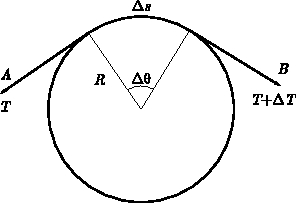
\includegraphics{figure/fig03.15}
	\caption{}
	\label{fig:03.15}
\end{wrapfigure}
表面,绳垂直于柱的母线,横断面如图\ref{fig:03.15}\;所示。设绳与圆柱间的静
摩擦系数为$\mu$,若绳一端$ A $的张力为$ T $,另一
端B的张力为$  T + \Delta T $。绳子刚刚要向$ B $端滑
动,这时的$  \Delta T  $等于多少?

\solution 考察绳段$ \Delta s $的受力及运动情况,把它的运动分解为切向
与法向。

在切向上所受的力为指向$ B $的$ T+\Delta T $及指向$ A $的$ T $,柱给绳的
摩擦力$ \mu P $指向$ A $,其中$ P $是$ \Delta s $给柱的正压力所以,由牛顿
% 107.jpg
第二定律,有
\begin{equation*}
    T + \Delta T - T - \mu P = 0
\end{equation*}
或\vspace{-1.56em}
\begin{equation*}
    \Delta T = \mu P
\end{equation*}

在法向上,所受的力有向心的是
$\left( T + \Delta T \right) _ \vec{r} = \left( T + \Delta T \right) \sin \dfrac{ \Delta \theta }{ 2 } \approx T \dfrac { \Delta \theta }{2}$及$ \left(T\right)_{\vec{r}} = T \sin \dfrac { \Delta \theta } { 2 } \approx T \dfrac { \theta } { 2 }$,
还有离心的是柱给绳
$ \Delta s $的力$ P $。所以,牛顿方程为
\begin{align*}
    F _ { \vec{r} } &= \sum _ i  F _ { n _ { i } } \\
    &= \left( T + \Delta T \right)_{\vec{r}} + \left( T \right)_{\vec{r}} - P \\
    &= \Delta m \frac { v ^ { 2 } } { R }
\end{align*}
其中$ m $为$ \Delta s $的质量,因为绳$ s $尚未滑动,所以,$  v \approx 0 $。因此得
\begin{equation*}
    \left( T + \Delta T \right) _{\vec{ r }} + \left( T \right) _{\vec{ r }} - P = 0
\end{equation*}
即\vspace{-1.56em}
\begin{equation*}
    T \Delta \theta - \frac { \Delta T } { \mu } = 0
\end{equation*}
或者\vspace{-1.56em}
\begin{equation*}
    \Delta T = \mu T \Delta \theta
\end{equation*}
在$ \Delta \theta \rightarrow 0 $的极限下,可得到
\begin{equation*}
    \dif T = \mu T \dif \theta
\end{equation*}

\example 如图\ref{fig:03.16}~所示,$ ABC $是质量为$ M $的劈形物体,高为
$ h $,静止放在光滑的水平面上,斜面$ AC $的倾角为$\theta $,顶端$ A $放一
质量为$ m $的小物体,自静止向下滑动,略去各面之间的摩擦。试
求:

(1) $ m $从斜面顶端滑到底时,$ M $的位移;

(2) $ m $下滑时,$ M $对地面的加速度$ a_1 $;

(3) $ m $对$ M $的加速度$ a'_2 $;

(4) $ m $对地面的加速度$ a_2$;

% 108.jpg
(5) $ m $与$ M  $之间的作用力$  N $;

(6) $ M $与桌面之间的正压力$ R $。
\begin{figurex}
	\centering
	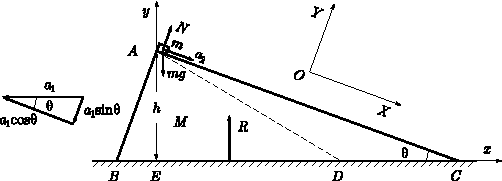
\includegraphics{figure/fig03.16}
	\caption{}
	\label{fig:03.16}
\end{figurex}

\solution 此题可有许多解法,下面我们只用惯性系中的牛顿第二
定律的基本方程求解。有了非惯性系知识(下一章)后,可以用非
惯性系方法再解一遍。

(1) $ m $的实际轨道是虚线$ AD $,$ ED $为$ m $的水平位移,$ CD $是$ M $的
水平位移。$ m $所受的力是$ mg $及$ N $,$ M $所受的力是$  M g  $, $ - N $ 及$ R $。
因此,在水平方向,$ m $与$ M $的牛顿方程为
\begin{align*}
    N \sin \theta &= m a _ { 2\text{水平} } \\
    N \sin \theta &= M a _ { 1 }
\end{align*}
由上两式得
\begin{equation*}
    \frac { C D } { E D } = \frac { a _ { 1 } } { a _ { 2\text{水平}}} = \frac { m } { M }
\end{equation*}
考虑到几何关系$  h = AC \cdot \sin \theta = BC \cdot \tg \theta  $,上式成为
\begin{align*}
    h &= \left( E D + D C \right) \tg \theta \\
    &= \left( \frac { M } { m } + 1 \right) D C \cdot \tg \theta
\end{align*}
因此当$ m $落到底时,$ M $走过的距离为
\begin{equation*}
    D C = \frac { h m } { M + m } \ctg \theta
\end{equation*}
% 109.jpg

(2) 由图\ref{fig:03.16},我们采用惯性系$ xEy $,利用加速度合成公式
\begin{equation*}
    \vec{a} _ { 2 } = \vec{a} _ { 1 } + \vec{a}' _ 2
\end{equation*}
由此,可得到下列$ m $的牛顿方程
\begin{align*}
    &N \sin \theta = m a _ { 2\text{水平} }  = m \left( a '_2 \cos \theta - a _ { 1 } \right) \\
    &m g - N \cos \theta = m a' _ { 2 } \sin \theta
\end{align*}
$ M $的牛顿方程是
\begin{equation*}
    N \sin \theta = M a _ { 1 }
\end{equation*}
求解上述三个方程就得到
\begin{equation*}
    \vec{a} _ { 1 } = - \frac { m g \sin \theta \cos \theta} { M + m \sin ^ { 2 } \theta } \vec{i}
\end{equation*}式中为x轴的单位矢量。
也可以用图\ref{fig:03.16}\;中的$ XOY $惯性系,则$ M $及$ m $的方程分别为
\begin{align*}
    &N \sin \theta = M a _ { 1 } \\
    &g \cos \theta - N = m a _ { 1 } \sin \theta
\end{align*}
求解后同样得到上述的$ a_1 $的表达式。

(3) 利用上述$\vec{a}_1$表达式,即可求出如下
\begin{equation*}
    a _ 2 ' = \frac { \left( M + m \right) \sin \theta } { M + m \sin ^ { 2 } \theta } g
\end{equation*}
它就是$ m $相对于M的加速度。

(4) $ m $对地面的加速度是
\begin{align*}
    a _ { 2 } &= \left( a _ { 2 }' \cos \theta - a _ { 1 } \right) \vec{i} - a _ 2 ' \sin \theta \vec{j} \\
    &= \frac { M \sin \theta \cos \theta } { M + m \sin ^ { 2 } \theta } g \vec{i} - \frac { \left( M + m \right) \sin ^ { 2 } \theta } { M + m \sin ^ { 2 } \theta } g \vec{j}
\end{align*}

(5) $ m $与$ M $之间的作用力$ N $为
\begin{equation*}
    N = \frac { M  m \cos \theta } { M + m \sin ^ { 2 } \theta } g
\end{equation*}

(6) 考虑$ M $在$ y $方向的力的平衡,即得$ M $与桌面之间的正压
力$ R $为

% 110.jpg
~\vspace{-1.56em}
\begin{align*}
    R &= M g + N \cos \theta \\
    &= \frac { M \left( M + m \right) } { M + m \sin ^ { 2 } \theta } g
\end{align*}
应当注意,当整个系统$  \left( M + m \right)  $在$ y $方向有加速度时,桌面给体
系的压力不再是$  \left( M + m \right) g  $,而是$ R $与$  \left( M + m \right) g  $之差提供了体系
在$ y $方向的加速度。